% Chapter Template

\chapter{FDTD - One-Dimensional Scenario} % Main chapter title

\label{Chapter2} % Change X to a consecutive number; for referencing this chapter elsewhere, use \ref{ChapterX}

This chapter will go more in depth into developing an application that can generate electromagnetic data in a one-dimensional domain. Previously, a series of steps to implement FDTD and that a part of them depend on the particular implementation was mentioned. A keen eye will notice moving forward, that while the code will not change too much, each implementation deserves a different approach in the theoretical sense.

%----------------------------------------------------------------------------------------
%	SECTION 1
%----------------------------------------------------------------------------------------

\section{1D Discretization}

The previous chapter concluded with the equations \ref{eqn:electricUpdateIntegral} and \ref{eqn:magneticUpdateIntegral}. They will now be used to do a FDTD discretization for the one-dimensional electromagnetic wave scenario. Throughout this section the update equations that will be used in the loops will be derived. Before moving on, Transverse modes must first be briefly discussed. A transverse mode is the type of pattern that an electromagnetic field, which is perpendicular with respect to the direction of the wave's propagation, has. For electromagnetic waves, the most relevant modes are TE (Transverse Electric) and TM (Transverse Magnetic). In this scenario, TEM mode will be used for discretization, meaning neither electric nor the magnetic field are moving in the direction of propagation.

%-----------------------------------
%	SUBSECTION 1
%-----------------------------------
\subsection{Spatial and Temporal Shift}

The first step of the FDTD discretization is a shift in spacetime of the electric and magnetic fields. This spatial shift is shown in Figure \ref{fig:fdtd1dDiscretized}.

\begin{figure}
	\centering
	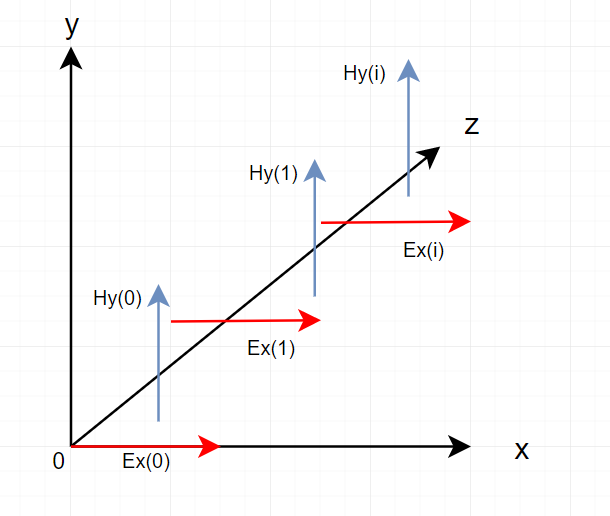
\includegraphics[scale=0.5]{Figures/fdtd1dDiscretized}
	\decoRule
	\caption[1D Spatial and Temporal Shift - TEM Mode]{The spatial and temporal shift of a one-dimensional electromagnetic scenario.}
	\label{fig:fdtd1dDiscretized}
\end{figure}

The electric vectors E are parallel to the x axis, while the magnetic vectors H are parallel to the y axis. The z axis in this case is the direction of the wave propagation.

%-----------------------------------
%	SUBSECTION 2
%-----------------------------------

\subsection{Electromagnetic Curls}

At first, the way that the vectors in Figure \ref{fig:fdtd1dDiscretized} are spaced out might seem odd. They look this way because they are part of each other's vector curl. There are two such curls in the one-dimensional scenario: one for the electric field vectors Ex,and one for the magnetic field vectors Hy. These curls are necessary for the update equations, because they explain the relationship between the electric fields and the magnetic ones.

\begin{figure}
	\centering
	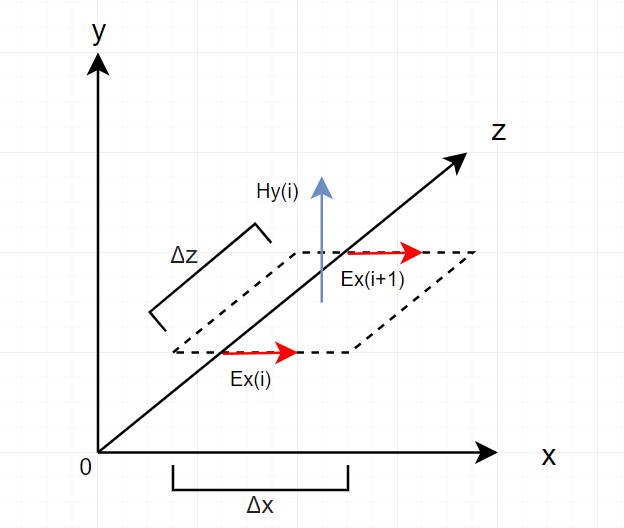
\includegraphics[scale=0.7]{Figures/fdtd1dHcurl}
	\decoRule
	\caption[1D Curl around $H_y$]{A graph showing the one-dimensional curl around the vector $H_y(i)$.}
	\label{fig:fdtd1dHcurl}
\end{figure}

Figure \ref{fig:fdtd1dHcurl} shows the curl around the magnetic vector $H_y(i)$. This curl can be used by plugging it in to the original equation \ref{eqn:electricUpdateIntegral}:

\begin{equation}
	\label{eqn:magneticCurl1}
	\oint E \cdot ds = E_x(i) \cdot \Delta x + E_z \cdot \Delta z - E_x(i+1) \cdot \Delta x - E_z \cdot \Delta z
\end{equation}

Since there is no Ez vector in the one-dimensional scenario, $Ez \cdot \Delta z = 0$. Therefore the equation \ref{eqn:magneticCurl1} can be simplified to:

\begin{equation}
	\label{eqn:magneticCurl2}
	\oint E \cdot ds = E_x(i) \cdot \Delta x - E_x(i+1) \cdot \Delta x
\end{equation}

On the left hand side of equation \ref{eqn:electricUpdateIntegral}:

\begin{equation}
	\label{eqn:magneticCurl3}
	\int \mu \cdot H \cdot dA = \mu \int H \cdot dA = \mu \cdot H_y(i) \cdot \Delta y \cdot \Delta z
\end{equation}

By combining \ref{eqn:magneticCurl2} and \ref{eqn:magneticCurl3}:

\begin{equation}
	\label{eqn:magneticCurl4}
	\Delta x(E_x(i) - E_x(i+1)) = -\frac{d}{dt} (\mu \cdot H_y(i) \cdot \Delta y \cdot \Delta z)
\end{equation}

\begin{equation}
	\label{eqn:magneticCurl5}
	E_x(i) - E_x(i+1) = -\mu \cdot \Delta z \cdot \frac{dH_y(i)}{dt}
\end{equation}

The  same thing can be done the for the curl of the electric vector $E_x$, shown in Figure \ref{fig:fdtd1dEcurl}, as follows (Similar to the previous scenario, $H_z = 0$):

\begin{figure}
	\centering
	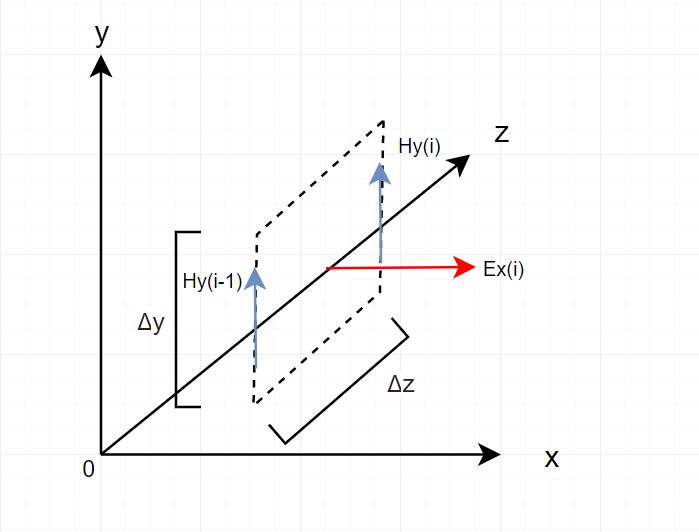
\includegraphics[scale=0.7]{Figures/fdtd1dEcurl}
	\decoRule
	\caption[1D Curl around $E_x$]{A graph showing the one-dimensional curl around the vector $E_x(i)$.}
	\label{fig:fdtd1dEcurl}
\end{figure}

\begin{equation}
	\label{eqn:electricCurl1}
	\oint H \cdot ds = H_y(i) \cdot \Delta y - H_y(i-1) \cdot \Delta y = \Delta y (H_y(i) - H_y(i-1))
\end{equation}

\begin{equation}
	\label{eqn:electricCurl2}
	\iint \epsilon \cdot E \cdot dA = \epsilon \cdot E_x(i) \cdot \Delta z \cdot \Delta y
\end{equation}

Combining \ref{eqn:electricCurl1} and \ref{eqn:electricCurl2}:

\begin{equation}
	\label{eqn:electricCurl3}
	\Delta y (H_y(i) - H_y(i-1)) = \frac{d}{dt} (\epsilon \cdot E_x(i) \cdot \Delta z \cdot \Delta y)
\end{equation}
\begin{equation}
	\label{eqn:electricCurl4}
	H_y(i) - H_y(i-1) = \epsilon  \cdot \Delta z  \cdot \frac{d}{dt} E_x(i)
\end{equation}

With those equations, one can now use the leapfrog time scheme to stagger these components along the time axis (Fig. \ref{fig:fdtd1dLeapfrog}).

\begin{figure}[!h]
	\centering
	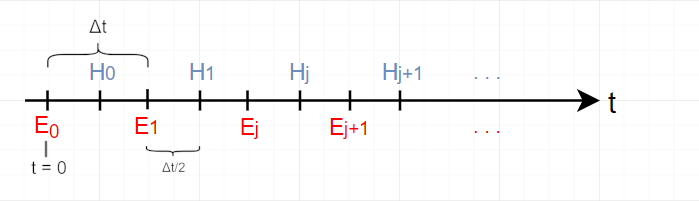
\includegraphics[scale=0.75]{Figures/fdtd1dLeapfrog}
	\decoRule
	\caption[Leapfrog Time Scheme]{Staggering the components along the time axis t using the leapfrog time scheme}
	\label{fig:fdtd1dLeapfrog}
\end{figure}

The following indexing scheme will be used:

\begin{equation}
	\label{eqn:indexingElectric}
	E_{i,j} = E(i \cdot \Delta z , j \cdot \Delta t)
\end{equation}

\begin{equation}
	\label{eqn:indexingMagnetic}
	H_{i,j} = H((i + \frac{1}{2}) \cdot \Delta z , (j + \frac{1}{2}) \cdot \Delta t)
\end{equation}

Using \ref{eqn:indexingElectric} and \ref{eqn:indexingMagnetic} results in the following time derivatives:

\begin{equation}
	\label{eqn:timeDerivativeE}
	\frac{d E_x}{dt} \bigg\rvert_{\underset{z = i \cdot \Delta z}{t=(j + \frac{1}{2})\Delta t}} = \frac{E_{x^{i,j+1}} - E_{x^{i,j}}}{\Delta t}
\end{equation}

\begin{equation}
	\label{eqn:timeDerivativeH}
	\frac{d H_y}{dt} \bigg\rvert_{\underset{z = (i + \frac{1}{2}) \Delta z}{t=j \cdot \Delta t}} = \frac{H_{y^{i,j}} - H_{y^{i,j-1}}}{\Delta t}
\end{equation}

Going back to equation \ref{eqn:magneticCurl5}:

\begin{equation}
	\label{eqn:timeDerivativeE2}
	E_x(i \cdot \Delta z) - E_x((i+1) \cdot \Delta z) = -\mu \cdot \Delta z \cdot \frac{d H_y((i+1/2)\Delta z) }{\Delta t}
\end{equation}

Evaluating at $t = j \cdot \Delta t$ gives:

\begin{equation}
	\label{eqn:timeDerivativeE3}
	E_{x^{i,j}} - E_{x^{i+1,j}} = -\mu \cdot \Delta z \cdot \frac{H_{y^{i,j}} - H_{y^{i,j-1}}}{\Delta t}
\end{equation}

Finally, by solving for ${H_{y^{i,j}}}$ one can get the update equation for the magnetic element:
	
\begin{equation}
	\label{eqn:magneticUpdate}
	H_{y^{i,j}} = H_{y^{i,j-1}} - \frac{\Delta t}{\mu \cdot \Delta z}(E_{x^{i,j}} - E_{x^{i+1,j}})
\end{equation}

In a similar way, the update equation for the electric element can be gotten by starting from the equation \ref{eqn:electricCurl4}. The result is:

\begin{equation}
	\label{eqn:electricUpdate}
	E_{x^{i,j+1}} = E_{x^{i,j}} + \frac{\Delta t}{\epsilon \cdot \Delta z}(H_{y^{i,j}} -  H_{y^{i-1,j}})
\end{equation}

Before moving on, it is critical to discuss the stability of the simulation, which relies on the value of $\Delta t$.

\subsection{Stability and Energy Conservation}\label{sec:stability}
Deciding the mesh size for a given domain is heavily based on the computational capabilities of the instruments that are being used, rather than the implementation itself. Therefore, it is fairly straightforward most of the time: one should make the mesh as small as possible, provided the implementation can finish computing within an amount of time that can be considered reasonable.

Unfortunately, this is not the case for the time step size, $\Delta t$. While it can be chosen arbitrarily, picking a number that is too large can cause the implementation to grow unstable (Figure \ref{fig:fdtd1dinstability}).

\begin{figure}[!h]
	\centering
	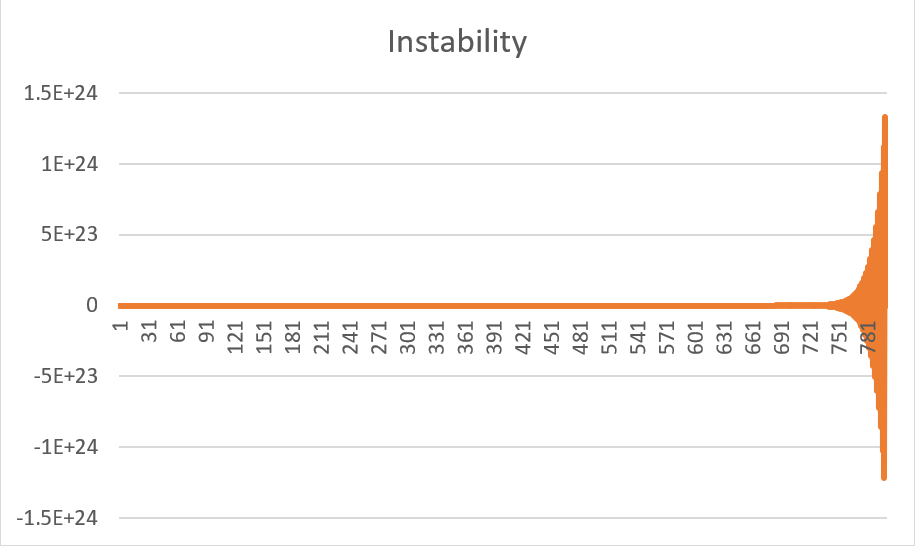
\includegraphics[scale=0.5]{Figures/fdtd1dinstability}
	\decoRule
	\caption[Instability]{The instability that can occur when choosing a $\Delta t$ number that is too high.}
	\label{fig:fdtd1dinstability}
\end{figure}

There is a max possible value for $\Delta t$ called $\Delta t_{max}$ that is derived from the Courant–Friedrichs–Lewy condition, which can be found using the following equation:

\begin{equation}
	\label{eqn:deltaTMax}
	\Delta t_{max} = \sqrt{\epsilon \cdot \mu} \cdot \frac{C_{max}}{\sqrt{(\frac{1}{\Delta x})^2 + (\frac{1}{\Delta y})^2 + (\frac{1}{\Delta z})^2}}
\end{equation}

The part with the deltas under the square root depends on the dimensions of the domain. Therefore, or this one dimensional scenario, equation \ref{eqn:deltaTMax} can be shortened to:

\begin{equation}
	\label{eqn:1DdeltaTMax}
	\Delta t_{max} = \sqrt{\epsilon \cdot \mu} \cdot \frac{C_{max}}{\sqrt{(\frac{1}{\Delta z})^2}}
\end{equation}

$C_{max}$ is a number that heavily depends on the method used after the main problem is discretized. In the case of explicit schemes such as FDTD, usually it is $C_{max} = 1$, meaning equation \ref{eqn:1DdeltaTMax} can be simplified further:

\begin{align}
	\label{eqn:1DdeltaTMaxFinal}
	\Delta t_{max} = \sqrt{\epsilon \cdot \mu} \cdot \frac{1}{\sqrt{(\frac{1}{\Delta z})^2}} \\
	\Rightarrow \Delta t_{max} = \sqrt{\epsilon \cdot \mu} \cdot \Delta z
\end{align}

So long as $\Delta t \leq \Delta t_{max}$, the implementation will stay stable. However, $\Delta_t$ also affects the amount of energy conservation in the system\textsuperscript{\cite{engle_skeel_drees_2005}}. During the course of a simulation the energy can fluctuate, thus deviating by the actual value by either increasing or decreasing in the long term. Such fluctuations do not occur in reality, therefore differing slightly. Symplectic integration schemes such as FDTD will feature a small, but constant, increase in energy the longer the simulation lasts. While there are ways to circumvent this problem\textsuperscript{\cite{gao2013optimal}}, they are outside the scope of this project.

%----------------------------------------------------------------------------------------
%	SECTION 2
%----------------------------------------------------------------------------------------

\section{C++ Implementation}

Calculating the update equations is by far the most difficult part of implementing FDTD. However, translating equations into code is not always straightforward. Before the implementation begins, one needs to prepare the coding environment. For this project, the author is using the Eclipse IDE for C++ Development\textsuperscript{\cite{eclipse}}. After the creation of a new project, the code file will start off with an empty skeleton that features the \textit{main()} method. Due to not needing any other classes, this is where all the code will be contained. Before that, one will need to include some standard C++ headers so that their methods, data types, and variables, can be used.

\begin{minted}[breaklines,frame=single,fontsize=\footnotesize]{c++}
#define _USE_MATH_DEFINES
	
#include <iostream>
#include <stdio.h>
#include <math.h>
#include <stdlib.h>
#include <cmath>
#include <vector>
#include <string>

using namespace std;
\end{minted}

To shortly explain what each line does:

\begin{itemize}
	\item \textbf{cmath, math.h}\textsuperscript{\cite{cmath}} - Header files that allow the use of various helpful math related commands and constants. Requires having \space \verb!#define _USE_MATH_DEFINES! set in order for everything to work properly
	\item \textbf{iostream, stdio.h}\textsuperscript{\cite{iostream}} - Allows for the usage of input and output stream objects and commands. In the 1D implementation, the program will print the data to the console by using \verb!cout!
	\item \textbf{stdlib.h}\textsuperscript{\cite{cstdlib}} - Provides helpful data types, especially when dealing with vectors
	\item \textbf{vector}\textsuperscript{\cite{vector}} - Arrays in standard C++ are not dynamic. Once populated, they can no longer be modified. That is why for this implementation vectors need to be used.
	\item \textbf{string}\textsuperscript{\cite{string}} - Includes the string datatype. A string is basically an array of characters. Not only can one use this to format the output more easily, it can also be very useful for printing debugging messages.
\end{itemize}

Next, some variables will need to be initialized. The permittivity $\epsilon$ and permeability $\mu$ of the domain that is going to be simulated need to be set first. For this scenario, the values for vacuum are going to be used, $\epsilon_{0}$ and $\mu_{0}$.

\begin{minted}[breaklines,frame=single,fontsize=\footnotesize]{c++}
const double permitivity = 8.854e-12;  // vacuum permitivity
const double permeability = 1.256e-6;  // vacuum permeability
\end{minted}

These numbers are normally infinite, therefore innacuracies are already being introduced into the simulation. For greater precision, one could include more decimals, though the difference for such a small case would still be negligible. It should be noted that although the units are not mentioned, all the calculations use standard SI units. This is important, as using the wrong unit could make the simulation inaccurate at best, or utterly unstable at worst.

\begin{minted}[breaklines,frame=single,fontsize=\footnotesize]{c++}
double L = 5;
int N = 200;
int iterNum = 800;
double deltaZ = L / N;
double deltaT = (deltaZ * sqrt(permitivity*permeability));
\end{minted}

\textbf{L} is the length of the domain in SI units, namely meters. \textbf{N} is the number of steps, or in the one-dimensional scenario the number of times the domain was split. \textbf{iterNum} is the number of iterations. \textbf{deltaZ} ($\Delta z$) is the difference between the current step and the next one in meters. This can be set to anything, but it would be desirable to evenly split the domain and the best way to do so would be to set it to a number that follows the pattern $x \cdot L/N$.

Special attention should be brought to \textbf{deltaT} ($\Delta t$). If this value is too big, the simulation will quickly grow unstable. While picking any arbitrary value would work, so long as it is small enough, one can choose a value that will always work through the equation below:

\begin{equation}
	\label{eqn:deltaTcode}
	\Delta t = \Delta z \cdot \sqrt{\epsilon \mu}
\end{equation}

This is the one-dimensional version of this equation. It will be seen how it changes later on when discussing the two-dimensional and three-dimensional scenarios. Now that the testing environment is ready, one will need to initialize the variables that will be used in these loops.

\begin{minted}[breaklines,frame=single,fontsize=\footnotesize]{c++}
// variables needed for Gaussian Pulse excitation
double eps = 1e-3;
double Teps = 50 * deltaT;
double beta = -(pow((2/Teps), 2) * log(eps));


vector<double> E;
vector<double> H;
vector<double> tE;
vector<double> tH;
\end{minted}

\textbf{E} and \textbf{H} are the electric and magnetic field vectors that will hold the data for each time step. For the one-dimensional scenario, in order to display the simulated data a time graph will be used, which is a graph of the values that an arbitrary point $n$ has during the simulation. A good choice  for this scenario would be the midpoint of the domain $N/2$, and the vectors \textbf{tE} and \textbf{tH} will contain the data of the electric and magnetic time graph respectively. It is also prudent to initialize some helpful values that will be used by the Gaussian pulse excitation, with the equation \ref{eqn:gaussianPulse} mentioned in chapter \ref{Chapter1}: \textbf{eps} ($\varepsilon$), \textbf{Teps} ($T_\varepsilon$), and \textbf{beta} ($\beta$), with equation \ref{eqn:gaussianBeta} that was discussed in the same chapter.

Now that the setup of the variables that will be needed for the simulation is done, it is time to actually move on to the \textit{main()} method where FDTD algorithm will be implemented. First, the magnetic and electric field vectors need to be populated, since this was not done as of yet. Since the simulation is going to have no initial charge in it, every point in these vectors can be initialized to $0$. Luckily there is a quick way to do so in C++ that does not require the use of loops:

\begin{minted}[breaklines,frame=single,fontsize=\footnotesize]{c++}
E.assign(N, 0);
H.assign(N, 0);
\end{minted}

This will push N zeros to the vectors. Now one will need to start looping for \mint{c++}{int i = 0; i < iterNum; i++} values. It can also be helpful to start off the Gaussian pulse here, by applying it to the beginning of the electric vector like so:

\begin{minted}[breaklines,frame=single,fontsize=\footnotesize]{c++}
double t = i * deltaT;
double gamma = Teps / 2;

E[0] = exp(-(beta * pow((t - gamma), 2)));
\end{minted}

Afterwards, by using the update equations that were derived above to get the values for the magnetic and electric fields:

\begin{minted}[breaklines,frame=single,fontsize=\footnotesize]{c++}
// loop for values
for (int z = 0; z < N-2; z++) {
	H[z] = H[z] - (deltaT / permeability / deltaZ) * (E[z] - E[z+1]);
}

for (int z = 1; z < N-1; z++) {
	E[z] = E[z] + (deltaT / permitivity / deltaZ) * (H[z] - H[z-1]);
}
\end{minted}

It should be noted that the starting index of a vector is zero, therefore when adding N values to these vectors, the index of the last value is going to be $N-1$. In these loops, this number must never be surpassed. For the magnetic vector H loop, it would need to stop when $z + 1 = N - 1 \Leftrightarrow z = N - 2$. Alternatively, one could also populate $N + 1$ values, and extend the domain one unit past the boundaries.

After the above update loops, but while still inside the main loop, the middle values will be stored into the respective time graph vectors for each time step:

\begin{minted}[breaklines,frame=single,fontsize=\footnotesize]{c++}
// time graph
tE.push_back(E[100]);
tH.push_back(H[100]);
\end{minted}

As mentioned previously, one can pick any point for this and it would still work. This is also another reasons why vectors are incredibly useful: since the vectors \textbf{tE} or \textbf{tH} were not populated with any values previously, they had a length of zero. However, using the \textit{push\_back()} method, the values can be added dynamically, therefore allowing to change the number of iterations at will. 

After running the main loop \textbf{iterNum} times, the values are finally printed as a comma separated list:

\begin{minted}[breaklines,frame=single,fontsize=\footnotesize]{c++}
cout << "\n\ntE\n";

// print E values
for (int n = 0; n < iterNum; n++) {
	cout << to_string(tE[n]) + ",";
}

cout << "\n\ntH\n";

// print H values
for (int n = 0; n < iterNum; n++) {
	cout << to_string(tH[n]) + ",";
}
\end{minted}

The result is shown in figure \ref{fig:fdtd1dconsole}.

\begin{figure}[h!]
	\centering
	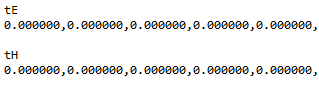
\includegraphics{Figures/fdtd1dconsole}
	\decoRule
	\caption[1D Console Output]{The console output of the FDTD one-dimensional algorithm}
	\label{fig:fdtd1dconsole}
\end{figure}

The time graphs can be considered to be the point of view that a single cell has throughout the simulation. While only effectively usable in the one-dimensional scenario, they provide an easier way to visualize moving simulations, due to being capable of showing all the data at once.

Now that the data was generated, it can finally be visualized.

\section{Data Visualization}

Generating the data was the difficult part. In order to visualize it into a form that is easily understandable by humans, a variety of programs can be used. An easy solution for this is Microsoft Office Excel\textsuperscript{\cite{excel}}. While this software requires a license, there are viable alternatives to it that should be able to achieve the same results.

For starters, the comma separated list that is in the console output, comprising of the data inside the time graph vectors for the midpoint of both magnetic and electric fields, needs to be copied to the first column, in the second row for the electric data and the third row for the magnetic data. This will populate the first cell for both rows. After that, one can go to \textbf{Data > Text to Columns} and then split the one cell list into multiple columns (\ref{fig:fdtd1dexcel1}).

\begin{figure}[h!]
	\centering
	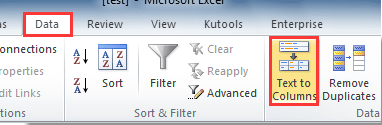
\includegraphics{Figures/fdtd1dexcel1}
	\decoRule
	\caption[1D Excel - Text to Columns]{Transforming data from a single cell containing the whole list, into separate columns for each value.}
	\label{fig:fdtd1dexcel1}
\end{figure}

After doing that for both electric and magnetic values, one can add a row of numbers above them for the timesteps. The result will look like so:

\begin{figure}[h!]
	\centering
	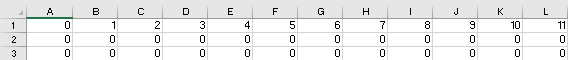
\includegraphics{Figures/fdtd1dexcel2}
	\decoRule
	\caption[1D Excel - Text to Columns]{Transforming data from a single cell containing the whole list, into separate columns for each value.}
	\label{fig:fdtd1dexcel2}
\end{figure}

\clearpage

With this, the data can be visualized however it is desired. For the purposes of this demonstration line graphs will be used. In Figure \ref{fig:emTimeGraph}, the time graph of the electric field was colored orange, and the magnetic field blue.

\begin{figure}[h!]
	\centering
	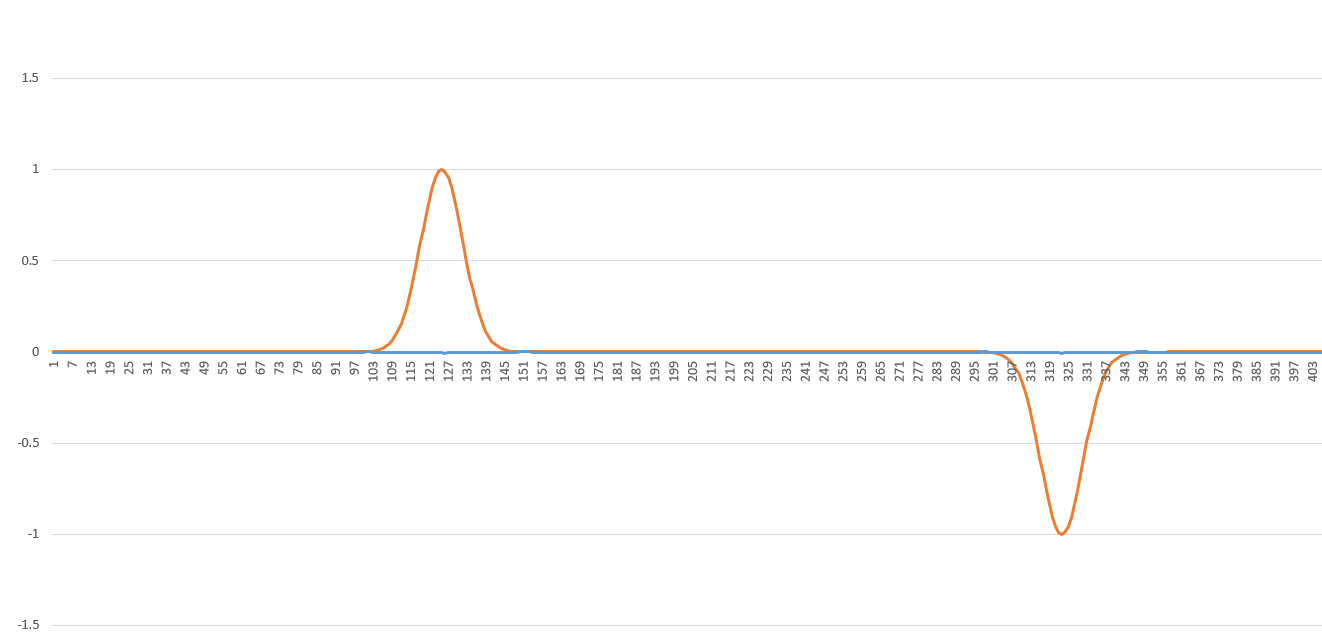
\includegraphics[height= 8cm,width=\textwidth]{Figures/1DtimeGraph1}\\
	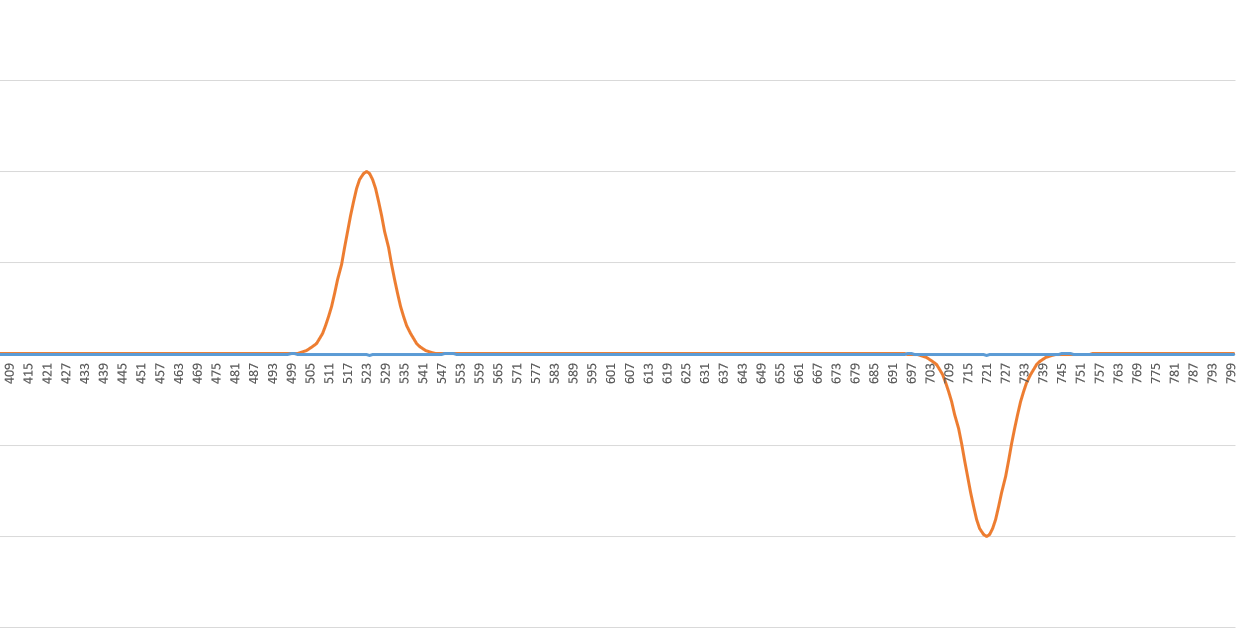
\includegraphics[height= 8cm,width=\textwidth]{Figures/1DtimeGraph2}
	\decoRule
	\caption[1D Electromagnetic Time Graph]{The time graph of the electromagnetic data generated by the 1D application.}
	\label{fig:emTimeGraph}
\end{figure}

\clearpage

It should be noted that both lines were shown in the same plane due to convenience. The waves themselves move as they did during the discretization done prior: electric waves move in the \textbf{X-Z} plane while the magnetic waves move in the \textbf{Y-Z} plane. Also, it can be noted that there is an enormous difference in the values of the electric and magnetic fields. One can easily tell that the electric wave is moving, but it is difficult to notice the magnetic wave movement. Here is one of those values zoomed in (Fig. \ref{fig:mTimeSnippet}):

\begin{figure}[H]
	\centering
	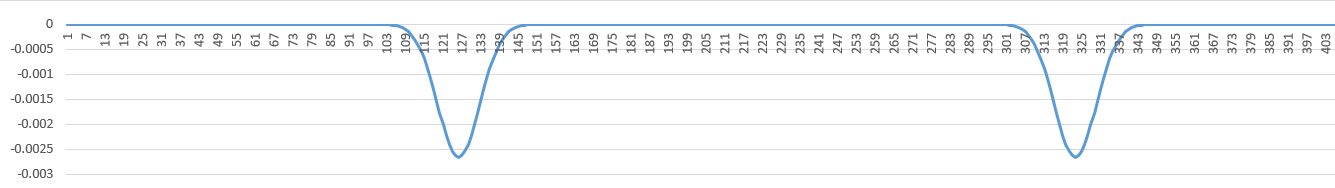
\includegraphics[height= 3cm,width=\textwidth]{Figures/1DmagneticTimeGraph1}
	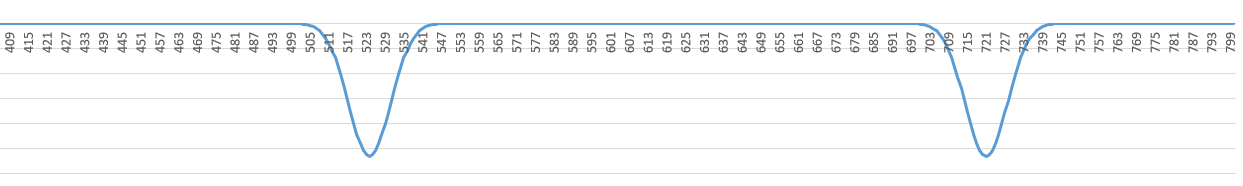
\includegraphics[height= 3cm,width=\textwidth]{Figures/1DmagneticTimeGraph2}
	\decoRule
	\caption[1D Magnetic Time Snippet]{A snippet of the time graph shown in Figure \ref{fig:emTimeGraph} zoomed in}
	\label{fig:mTimeSnippet}
\end{figure}

The reason for this difference being so big is due to the medium chosen for this domain: free space or otherwise known as vacuum. Also known as the impedance of free space, this value is commonly known as $Z_0 = $ \SI{376.730313668(57)}{\ohm}. This is also the ratio between the electric field and the magnetic one in free space. The value can also be calculated by using the permittivity and permeability:

\begin{equation}
	\label{eqn:impedance}
	Z_0 = \frac{E}{H} = \sqrt{\frac{\mu_0}{\epsilon_{0}}}
\end{equation}

Something else worth noting is the distance between each wave. If the midpoint is chosen as the observation point for the values of the time graph, the distance between the starting point of each wave will be precisely $N$, the size of the domain. If one decided to use a different point of observation, the distance between each wave would vary. However, the distance between the first wave and the fourth, the second and the fifth, and so on, would always be $N \cdot 2$. 

Next comes the two-dimensional scenario.
	